
%----------------------------------------------------------------------------------------
%	MLA
%----------------------------------------------------------------------------------------

\chapter{MLA Style} 


\section{Formatting the MLA essay}
When setting up your word processor for an MLA-formatted document, use the 
following settings:

\begin{itemize}
\item Set one-inch margins on all sides of the document.
\item Double-space the entire document, including block quotes.
\item In the top left portion of the first page, type your name, instructor's name, course title, and date on separate, double-spaced lines.
\item Include your last name and a page number on each page in the top right corner of the header.
\item Include a centered title on the first page.
\item Indent the first line of each paragraph with a tab set to 1/2 inch.
\end{itemize}

\newpage



When a quotation runs more than four typed lines, use a \textbf{block quote}. A block quote is a free-standing block of text, set apart from the rest of the text. When formatting blockquotes in MLA, use the following rules: 

\begin{itemize}
\item Begin the block quote on a new line. 
\item Indent every line of the quote 1 inch from the left margin (this should be two tabs). 
\item Do not use quotation marks around the quoted material. 
\item Place the parenthetical citation \emph{after} the final punctuation of the quoted passage.
\end{itemize}

\newpage
\section{MLA page example}

\bigskip

\begin{tcolorbox}[enhanced,width=4.2in,left=.3in, right=.3in,
   drop fuzzy shadow southeast,
    boxrule=0.4pt,sharp corners,colframe=black!80!black,colback=white!10]

\medskip

{\scriptsize \begin{flushright} Tate 9 \end{flushright}
\begin{doublespacing}
Rufus Tate

Close Reading

9/25/16

Prof. Moon

\begin{center}Emily Dickenson's Poem \#365 \end{center}
\hspace{1.4em} Emily Dickinson's poem \#365 opens with an unequivocal, affirmative declaration pertaining to the existence of God.  Yet, as the poem progresses, the religious conviction displayed in the opening categorical statement "I Know that He Exists" gradually abates until finally transforming into a frantic consideration of the possibility that the life of faith is but a cruel hoax.  The poem's transition from an unswerving certainty, modeled in the opening line's declarative sentence, to the disconcerting and telling ambiguity of the final stanzas therefore compactly summarizes a loss or crisis of religious faith in the speaker.  
  
\hspace{1.4em} The opening line of the poem, "I know that He exists," reads like a statement of scientific fact.  Rather than proffer a statement of faith (a belief in things unseen), the speaker first envisions the problem of God's existence as something resolvable by the operation of reason.  The speaker's resolute claim that she "know[s]" God exists reveals that the issue has been definitively concluded by way of a previous--though unidentified--process of  reasoning.  The unbroken line and full stop, along with the statement's uncompromising, declarative nature, conspire to give the poem's opening line and its assertion about the existence of God the status of unassailable truth.  

\hspace{1.4em}In the following lines of the first stanza, however, the speaker's lack of any real or tangible evidence for her claim becomes apparent, invalidating the former, putatively empirical, understanding of God's existence.  

\end{doublespacing}}
\bigskip


\end{tcolorbox}

%\vspace*{\fill}
%\begin{center}
%\begin{center}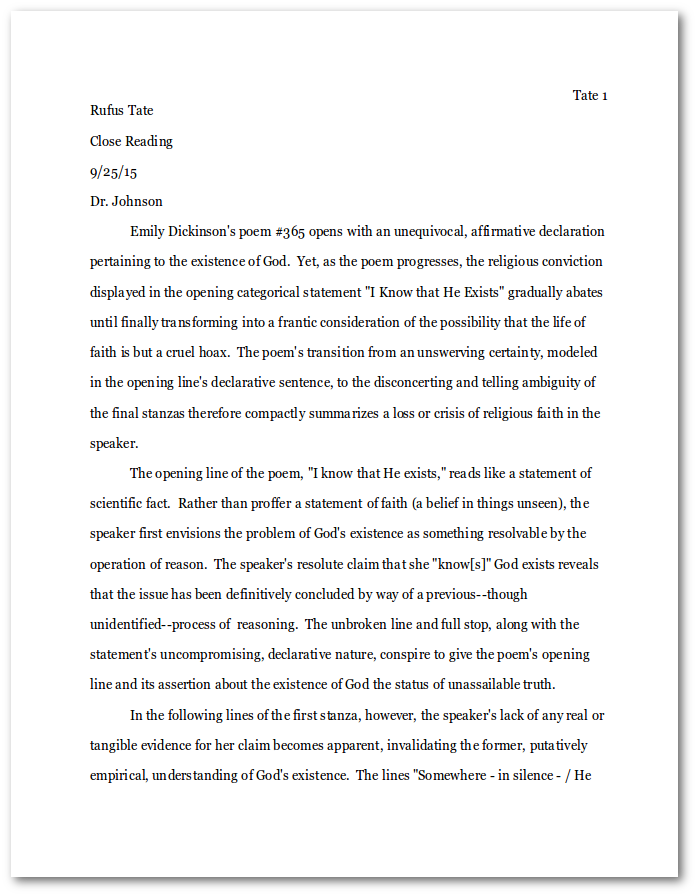
\includegraphics[width=.49\textwidth]{mlastyle}\end{center}
%\end{center}
%\vspace*{\fill}

\newpage
\section{MLA block quote example}
%\vspace*{\fill}
%\begin{center}
%\begin{center}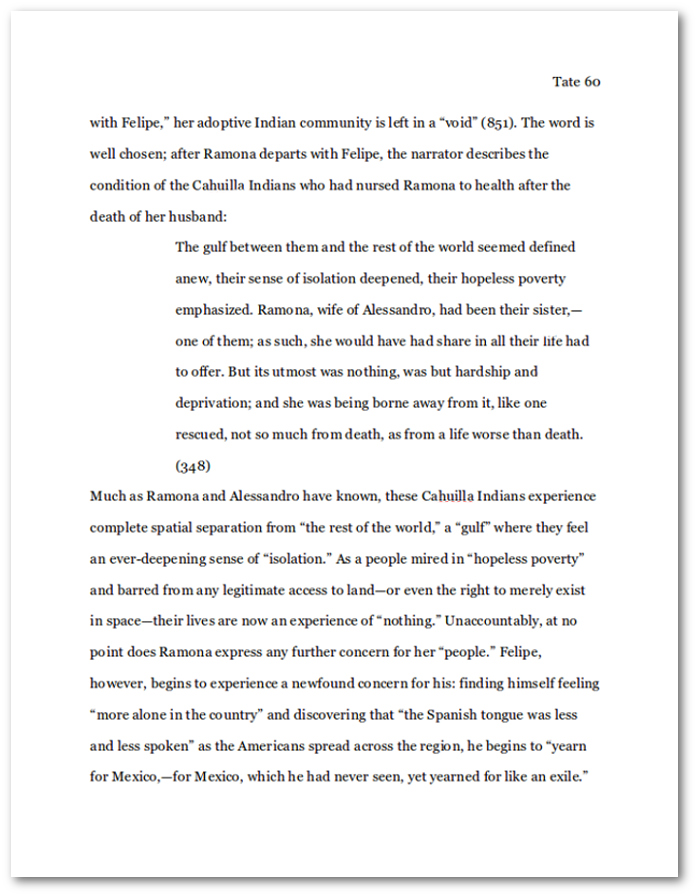
\includegraphics[width=.49\textwidth]{mlablockquote}\end{center}
%\end{center}
%\vspace*{\fill}

\bigskip

\begin{tcolorbox}[enhanced,width=4.2in,left=.35in, right=.35in,
   drop fuzzy shadow southeast,
    boxrule=0.4pt,sharp corners,colframe=black!80!black,colback=white!10]

\medskip

{\scriptsize \begin{flushright} Tate 29 \end{flushright}
\begin{doublespacing}
frequently result in absurdities; an illustration of which may be found in Janie Hinds' 2004 essay on the novel, where she argues the following:
\begin{myenv}The historical Walking Purchase Treaty of 1737, the ‘‘encroachment’’ event alluded to in Edgar Huntly as taking place 30 years before the events of the novel, stipulated that English settlers would own as much territory as they could walk in a day; when the English hired professional runners to cover at least three times as much ground as a person could legitimately cover in walking, the Delaware became understandably hostile, not only about the loss of territory but about the colonists’ trick. (335)\end{myenv}
Hinds here refers to an important moment in the novel when Edgar Huntly explains that the Delaware who formerly lived in the region left due to the “perpetual encroachments of the English colonists” (198). Although Huntly does remark that the departure of the Delaware tribe took place “about thirty years ago,” the event should in no way be confused with the Walking Purchase. Since the novel's setting is almost universally accepted to be in the year 1787, the “encroachments” mentioned by Edgar Huntly must have occurred in, or around, the year 1757—two decades \emph{after} the Walking Purchase. In her attempt to preserve this historical gloss, therefore, Hinds effectively relocates the novel's setting two decades into the past—a claim that contravenes virtually all historical scholarship on the novel and potentially muddles our understanding of the root causes of the native violence in Huntly's narrative. Although the memory of this dishonorable theft of land is undeniably a powerful explanation of the Delaware's revanchist violence within the novel (an argument made by many scholars), we do ourselves a disservice to ignore Brown's plain attempts to have us view his narrative as a statement on “recent incidents.”

\end{doublespacing}}

\bigskip
\smallskip
\smallskip

\end{tcolorbox}



\newpage

\section{In-text citations}
The MLA style uses parenthetical citations to indicate the author and page number of sources. These parenthetical citations take two forms. The first form is used when the source you are citing \emph{is known or understood} by your audience. The second form is used when the author being cited is \emph{unknown or unclear}. In the following sentence, the author of the source in question is obvious. Since the author is known to the reader, the citation uses \textbf{only the page number} of the source: 

\begin{quote}
According to scholar James Frey, "Americans eat five pounds of ice cream 
annually" (78).
\end{quote}

\noindent In the following versions of the sentence, however, the author is not stated:

\begin{quote}
According to one scholar, "Americans eat five pounds of ice cream annually" (Frey 78).
\end{quote}

\noindent Or:
\begin{quote}
Studies have shown that the American people consume an average of five pounds of ice 
cream every year (Frey 78).
\end{quote}

\noindent In the first sentence, the author is referred to only as a generic "scholar." To give the reader information on which scholar is being cited, Frey's name is included in the citation. In the second sentence, the author describes the report, not its author; as a result, the student has included Frey's name to indicate whose report is being referenced. 

%----DONE-----------

\section{List of Works Cited}

MLA requires a bibliography at the conclusion of the essay that includes the full 
citation of the sources cited within the essay. In MLA, the bibliography is known as the 
\textbf{Works Cited} page. When setting up a Works Cited page, use the following rules and 
characteristics:

\begin{itemize}
\item Center the words "Works Cited" at the top of the page.
\item Use your last name and the page number on the right side of the page's header.
\item Double space the Works Cited entries.
\item Alphabetize the entries by the author's last name.
\item If an entry runs more than one typed line, indent the second (and any subsequent) line with a 1/2-inch tab.
\item If two or more works by the same author are used, list the entries alphabetically by title. After the first entry, replace the author's name with three dashes followed by a period.
\end{itemize}
\newpage

\section{Works Cited example}
%\begin{center}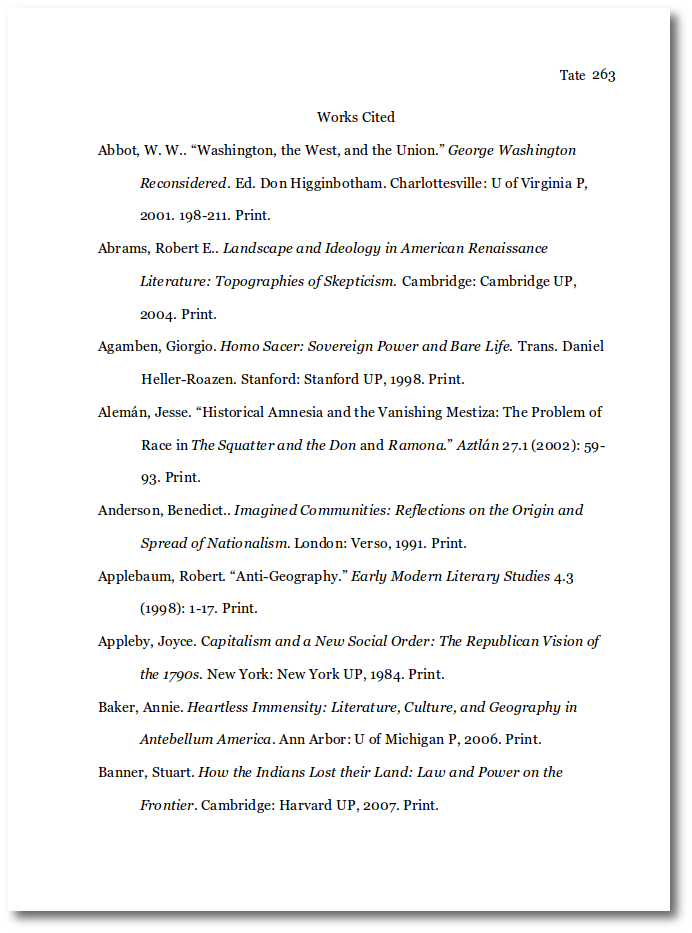
\includegraphics[width=.48\textwidth]{mlaworkscited}\end{center}

\bigskip

\begin{tcolorbox}[enhanced,width=4.2in,left=.3in, right=.3in,
   drop fuzzy shadow southeast,
   halign=flush left,
    boxrule=0.4pt,sharp corners,colframe=black!80!black,colback=white!10]

\medskip

{\scriptsize \begin{flushright} Taylor 9 \end{flushright}

\begin{center}Works Cited \end{center}
\begin{doublespacing}
\hangindent3em{
Abrams, Robert E. \emph{Landscape and Ideology in American Renaissance Literature: Topographies of Skepticism}. Cambridge: Cambridge UP, 2004. Print.}

\hangindent3em{Abrams, Robert E.. Landscape and Ideology in American Renaissance 	Literature: Topographies of Skepticism. Cambridge: Cambridge UP, 2004. Print.}

\hangindent3em{Alemán, Jesse. “Historical Amnesia and the Vanishing Mestiza: The Problem of Race in \emph{The Squatter and the Don} and \emph{Ramona}.” \emph{Aztlán} 27.1 (2002): 59-93. Print.}

\hangindent3em{Anderson, Benedict. \emph{Imagined Communities: Reflections on the Origin and Spread of Nationalism}. London: Verso, 1991. Print.}

\hangindent3em{Baas, Robert. “Anti-Geography.” \emph{Early Modern Literary Studies} 4.3 (1998): 1-17. Print.}

\hangindent3em{Bjorn, Joyce. \emph{Capitalism and a New Social Order: The Republican Vision of 	the 1790s}. New York: New York UP, 1984. Print.}

\hangindent3em{Carver, Annie. \emph{Grave Dangers: Spirits and Hauntings in the American Renaissance}. Ann Arbor: U of Michigan P, 2006. Print.}

\hangindent3em{Graves, Stuart. \emph{How the Indians Lost their Land: Law and Power on the Frontier}. Cambridge: Harvard UP, 2007. Print.}

\hangindent3em{Hill, William. \emph{History of the Blue Ridge}. New York: Dobbs Publishing, 1987. Print.}

\hangindent3em{
Kleiner, Randy. \emph{Escaping the Redneck Riviera}. Atlanta: Peach Publishing, 1988. Print.
}

\hangindent3em{Linter, Fred. \emph{The Theory of Landscape}. Boston: Boston UP, 1999. Print.
}

\end{doublespacing}}

\bigskip
\bigskip

\end{tcolorbox}


\newpage



\section{The MLA bibliography}

The following section provides examples for citing sources that are commonly found in
academic writing. The various forms have been organized into sections on \textbf{books}, \textbf{periodicals}, \textbf{electronic sources}, and \textbf{other types of sources} that are less common.


\section{Book forms}

\subsection{A book by one author}

\hangindent1.2cm{
{\color{Ahrenge}Last Name, First Name. \emph{Title}. City: Publisher, Year. Medium of Publication.
}}

\hangindent1.2cm{
Taylor, Herman. {\emph{A Tale of One City}}. New York: Little and Sons, 1998. Print.
}
 
\subsection{Two or more works by the same author(s)}

\hangindent1.2cm{
San, Rathanak. \emph{Escaping Vietnam}. Atlanta: Peach Publishing, 1988. Print.
}
\medskip

\hangindent1.2cm{
- - -. \emph{The Golden Triangle}. New York: Gray and Long, 1999. Print.}

\begin{itemize}\item If you cite two works by the same author, use the author's first and last name in the first instance. For any additional works by the same author, use three dashes followed by a period in place of the author's name. Place the works in alphabetical order using the first important word in the title.\end{itemize}

\subsection{Two or three authors}


\hangindent1cm{
Roberts, John, Philip Glass and Jane Hinds. \emph{Recovering the City of Boston}. Boston: U of Massachusetts P, 2000.}

\begin{itemize}\item Cite the first author using the typical Last Name, First Name format. For each subsequent author, use First Name Last Name.\end{itemize}

\subsection{Four or more authors}


\hangindent1.2cm{
Bankston, Jonathan, et al. \emph{On Barns}. Bourne: Woodcraft Publishing, 2013. Print}

\begin{itemize}\item If a work has four or more authors, you may give the first author's name and then replace the other authors with the Latin term "et al," which means "and others." \end{itemize}

\subsection{A book with an editor}
\hangindent1.2cm{
James, Henry. \emph{Portrait of a Lady}. Ed. Leon Edel. Boston: Houghton, 1963. Print.}

\begin{itemize}\item If a work has multiple editors, use Eds. followed by the editors' names in the order they are listed in the source. \end{itemize}


\subsection{An edition (other than the first)}
\hangindent1.2cm{
Thompson, Fred. \emph{Why I Fight}. 3rd ed. New York: Vanity Publications, 2000. Print.}

\subsection{A republished book}

\hangindent1.2cm{

{\color{Ahrenge}Last Name, First Name. \emph{Title}. Original Year of Publication. City of Publication: Publisher, Year of Publication. Medium of Publication.}}

\hangindent1.2cm{
James, Esther. \emph{My Life}. 1946. New York: Random House, 2001. Print.}

\begin{itemize}\item A republished book is one that was previously published in a different form, perhaps even from a different publisher. For books of this kind, indicate the original year of publication after the title. \end{itemize}

\subsection{Corporate author (written by organization or government)}


\hangindent1.2cm{
John Bigam Society. \emph{The Religions of Kenya}. New York: Nairobi Publishing, 2000. Print.}

\medskip 

\hangindent1.2cm{
United States. Dept. of Transportation. \emph{State Highway Sinage Regulations}. Washington: GPO, 2002. Web.}

\begin{itemize}\item If the author of a work is a government or institution, use the name of that organization in place of the author. If the text is the publication of a government, include the name of the department or agency. \end{itemize}

\subsection{An anthology}
\hangindent1.2cm{
Foner, Eric, ed. \emph{An American Voice: A Collection of America's Finest} \emph{Essays}. Boston: McKinley and Smith, 2011. Print.}

\subsection{Work in an anthology or collection of essays}
\hangindent1.2cm{
Graves, Thomas. "The History of our National Anthem." \emph{An American Voice: A Collection of America's Finest Essays.} Ed. Eric Foner. Boston: McKinley and Smith, 2011. 20-41. Print.}

\subsection{No author or editor}

\hangindent1.2cm{
\emph{A Guide to Boston}. Boston: Beantown Publishing, 2000. Print.}

\subsection{Forward, introduction, preface, or afterward}

\hangindent1.2cm
{Knox, John. Introduction. \emph{The Life of James}. By Elders Johnson. New York: Random House, 2009. 1-8. Print.}

\subsection{A book with a translator} 
\hangindent1.2cm{
McDougle, Astrid. \emph{The Basics of Gaelic}. Trans. Paddy Maloney. New York: Vintage, 1990. Print.}

\subsection{Multivolume work}

\hangindent1.2cm{Graves, Johanna. \emph{Ronald Reagan and the Iran-Contra Affair}. Vol. 7. New York: Greenstalk, 1988. Print.}

\subsection{Book in a series}


\hangindent1.2cm{
Smith, Rod, ed. \emph{American Economic Expansion in the Gilded Age}. By Andrew Stills. New York: Grim and Drang, 1988. Print. American Economics.}

\begin{itemize}\item If a book is part of a published series, indicate the name of the series at the conclusion of the citation. \end{itemize}

\subsection{Dictionary or encyclopedia entry}

\hangindent1.2cm{
"Suzerian." \emph{Merriam-Webster's Collegiate Dictionary}. 10th ed. 2008. Print.}

\subsection{Sacred text}

\hangindent1.2cm{
\emph{The Holy Bible, King James Version}. New York: American Bible Society, 1999.}

\begin{itemize}\item For sacred texts such as the Bible, Koran, or Torah. If you are citing a particular
edition, include that information.\end{itemize}


\subsection{Book with title within the title}


\hangindent1.2cm{
Hixson, Fred. \emph{On Cormac McCarthy's }Blood Meridian. New York: Plainspeak Press, 2000.}

\begin{itemize}\item If a book title contains the title of another book, remove the italics to indicate the title
of the other work. \end{itemize}
%--------------------------------------------------------------------------------------------
%Periodicals
%-------------------------------------------------------------------------------------------


\section{Periodical forms}

\subsection{Article in a scholarly journal with volume and issue numbers}
\hangindent1.2cm{
Taylor, James. "The Indian Matter of Charles Brockden Brown's \emph{Edgar Huntly}." \emph{American Literature} 45.6 (1998): 432-45. Print.}

\subsection{Article in a scholarly journal with only volume numbers}
\hangindent1.2cm{
Johnston, Johanna. "A Reading of \emph{Moby Dick}." \emph{North Dakota Quarterly} 45 (1978): 45-56. Print.}

\subsection{Article in a newspaper}
\hangindent1.2cm{
McKinley, Robert. "Cat Saved from Dog." \emph{New York Times} 7 Oct. 2011: A12+. Print.}

\begin{itemize}\item When an article appears on nonconsecutive pages, indicate the section where article begins 
then use a + sign. \end{itemize}

\subsection{Editorial in a newspaper}
\hangindent1.2cm{
"How to Reduce Crime." \emph{Sunapee Lake Times} 13 Nov. 2012: A4. Print.}

\subsection{Letter to the editor of a newspaper}
\hangindent1.2cm{
Johnson, Smitty. "Reduce our Property Taxes." Letter. \emph{Henniker Telegraph} 14 Oct. 2013: A1. Print.} 

\subsection{A review}
\hangindent1.2cm{
Smith, James. Rev. of \emph{The Orchard Revival}, by Cormac Freedman. \emph{Oregon Magazine} 23 Oct. 2011: 34-36. Print.} 

\subsection{An unsigned article in a newspaper}
\hangindent1.2cm{
"A Walk Down Nostalgia Lane." \emph{Bloomington Sun} 28 Oct. 2013: B6. Print.}

\subsection{Article in a magazine}
\hangindent1.2cm{
Smith, Jim. "Remembering Tony." \emph{New Yorker} Jan. 2010: 12-18. Print.}


%--------------------------------------------------------------------
\section{Online sources}

\subsection{Article in an online database}


\hangindent1.2cm{
Taylor, Abel. "\emph{Moby Dick} and the Cold War." \emph{American Literature} 45.6 (2010): 45-57. JSTOR. Web. 12 July 2012.}

\begin{itemize}\item Cite the source as you would a print article then include the database name, medium of access, and date of access. \end{itemize}

\subsection{An entire website} 
\hangindent1.2cm{
Zimmerman, Constantine. \emph{The Moose Report}. New Hampshire Hiking Club, 2013. Web. 13 March 2013.}


\subsection{A work from a website}
\hangindent1.2cm{
Reagan, John. "The Judo Champion Parent." \emph{Parenthood Online}. Ed. Jessie McCarver. The Parent Institute of Boston. Oct. 2011. Web. 5 Oct. 2012.}

\subsection{Online book or book chapter}
\hangindent1.2cm{
Melville, Herman. \emph{Moby Dick}. New York: RP Johnson, 1864.\\ Bartleby.com. Web. 7 Nov. 2000.}


\subsection{Article in an online scholarly journal}
\hangindent1.2cm{
Nelson, Grady. "Electronic Literature Comes of Age." \emph{e-Lit Quarterly}. 8.2 (2012): n. pag. Web. 28 Oct. 2013.}

\begin{itemize}\item Some scholarly journals that are only published online do not use page numbers for their articles. In this case, use "n.pag." in place of the page number range. \end{itemize}

\subsection{Article in an online newspaper}
\hangindent1.2cm{
Taylor, Robert C. "Harvesting Undersea Sponges." \emph{New York Times}. New York Times, 23 Nov. 2000. Web. 10 Dec. 2012.}


\subsection{Article in an online magazine}
\hangindent1.2cm{
James, Brian Taylor. "The New War on Terror." \emph{Foreign Affairs Monthly}. Errata Publishing, 2 Oct. 2009. Web. 12 Nov. 2012.}


\subsection{Blog entry}
\hangindent1.2cm{
Hardeman, Chad. "The Recent Healthcare Debate." \emph{The Health Blog}. 4 July 2010. Web. 12 Dec. 2010.}



%Online editorial
%Online film review

\subsection{Email}

\hangindent1.2cm{
Cooledge, John. "My Election Thoughts." Message to the author. 12 Nov. 2012. Email.}


%Posting from an online discussion board

\subsection{Article from an online reference work, such as Wikipedia}
\hangindent1.2cm{
"Al-Qaeda." Wikipedia. Wikimedia Foundation, 3 April 2004. Web. 12 Oct. 2013.}



\subsection{Podcast:}
\hangindent1.2cm{
Zeender, Nathan and Michael Tonsmeire. "Dark Lagers." James Spenser. \emph{Basic Brewing Radio}. 31 Jan. 2013. Web. 12 Mar. 2013.}

\section{Other types of sources}

\subsection{A dissertation}
\hangindent1.2cm{
Redburn, Marcus. "A Study of Melville's Aesthetics." Diss. Boston University, 1978.}

\subsection{An advertisement}
\hangindent1.2cm{
Dove Body Wash. Advertisement. \emph{Fortune Monthly} Oct. (2012): 23. Print.}


\subsection{Artwork}
\hangindent1.2cm{
Freeman, Dianna. \emph{Still Life 7}. Watercolor. 2009. Hunter Museum of Art, Chattanooga.}

\begin{itemize}\item For a work of art, include the medium after the title. For example: photograph, oil on canvas, watercolor, mixed media. \end{itemize}

\subsection{Film or video clip}
\hangindent1.2cm{
\emph{Rushmore}. Dir. Wes Anderson. Perf. Bill Murray, Jason Schwartzman, and Olivia Williams. Buena Vista International, 1998. DVD.}

\begin{itemize}\item Include the lead performers in the film after the director. \end{itemize}


%Broadcast interview
%Published interview
%Unpublished letter
%Published letter
%Map or chart
%Musical score
%Sound recording
%Oral presentation
%Paper from a conference
%Performance
%Television or radio program
%Pamphlet, brochure, or press release
%Legal source
%A digital file, such as .mp3, .pdf, etc.

%----------------------------------------------------------------------------------------
% END OF SECTION
%----------------------------------------------------------------------------------------